\documentclass[french, 9pt]{article}

%-------------------------------------------------------------------------------
\usepackage[a4paper,top=1cm,bottom=1cm,left=1cm,right=1cm,marginparwidth=0.5cm]{geometry}
\usepackage{amsmath,amsfonts,amssymb,amsthm}
\usepackage[french]{babel}
\usepackage[utf8]{inputenc}
\usepackage[T1]{fontenc}
\usepackage{enumerate}
\usepackage{natbib}
\usepackage{graphicx}
\usepackage{xspace}
\usepackage{color,xcolor}
\usepackage{tikz}
\usepackage{remreset}
\usepackage{url}
\usepackage{boites}
% \usepackage{extsizes} % Permet \documentclass[french, 14pt]{extreport}
% \usepackage[a4paper,top=1cm,bottom=2cm,left=1cm,right=1cm,marginparwidth=.75cm]{geometry}
% \usepackage{minitoc}

\graphicspath{{../Figures/}}
% Environnement
\newtheorem{theorem}{Théorème}
\newtheorem{definition}{Définition}
\newtheorem{lemma}{Lemme}
\newtheorem{proposition}{Proposition}
\newtheorem*{theorem*}{Théorème}
\newtheorem*{definition*}{Définition}
\newtheorem*{proposition*}{Proposition}
\newtheorem*{corollary*}{Corollaire}
\newtheorem*{assumption*}{Hypothèse}
\newtheorem*{algorithm*}{Algorithme}
\newtheorem*{lemma*}{Lemme}
\newtheorem*{remark*}{Remarque}
\newtheorem*{exercise*}{Exercice}
\newtheorem{exercise}{Exercice}
\newcommand{\remark}{\bigskip\noindent\textbf{\textsl{Remarque.}}\xspace}
\newcommand{\remarks}{\bigskip\noindent\textbf{\textsl{Remarques.}}\xspace}
\newcommand{\parSR}[1]{\paragraph*{\textsl{#1}}\xspace}
\renewcommand{\proof}{\bigskip\noindent\underline{\textsl{Démonstration}.}\xspace}
\newcommand{\eproof}{$\blacksquare$}

% Effets, couleurs
\newcommand{\emphase}[1]{\textcolor{red}{#1}}
\newcommand{\demoProp}[1]{\noindent{\textbf{\textsl{Démonstration de la proposition \ref{#1} :}}}}
\newcommand{\itemdot}{\textbullet}

% Moments
\DeclareMathOperator{\Esp}{\mathbb{E}}
\DeclareMathOperator{\diag}{diag}
\DeclareMathOperator{\Cov}{\mathbb{C}ov}
\DeclareMathOperator{\tr}{tr}
\DeclareMathOperator{\Var}{\mathbb{V}}
\let\Pr\relax\DeclareMathOperator{\Pr}{\mathbb{P}}
\renewcommand{\d}{\text{d}}

% R, N, ...
\newcommand{\cst}{\text{cst}}
\newcommand{\Cbb}{\mathbb{C}}
\newcommand{\Ibb}{\mathbb{I}}
\newcommand{\Nbb}{\mathbb{N}}
\newcommand{\Rbb}{\mathbb{R}}
\newcommand{\Zbb}{\mathbb{Z}}

% Indicateurs

% Lois et ensembles
\newcommand{\Acal}{\mathcal{A}}
\newcommand{\Bcal}{\mathcal{B}}
\newcommand{\Ccal}{\mathcal{C}}
\newcommand{\Ecal}{\mathcal{E}}
\newcommand{\Gcal}{\mathcal{G}}
\newcommand{\Ical}{\mathcal{I}}
\newcommand{\Lcal}{\mathcal{L}}
\newcommand{\Mcal}{\mathcal{M}}
\newcommand{\Ncal}{\mathcal{N}}
\newcommand{\Pcal}{\mathcal{P}}
\newcommand{\Rcal}{\mathcal{R}}
\newcommand{\Scal}{\mathcal{S}}
\newcommand{\Ucal}{\mathcal{U}}
\newcommand{\Xcal}{\mathcal{X}}
\newcommand{\Ycal}{\mathcal{Y}}

% Comments
\newcommand{\SR}[2]{\textcolor{gray}{#1}\textcolor{red}{#2}}
\newcommand{\todo}[1]{\textcolor{red}{\`A faire~: {\sl #1}}}
\newcommand{\dessin}[1]{
\begin{center}\framebox{\begin{minipage}{\textwidth}
  \textcolor{purple}{#1}
\end{minipage}}\end{center}
\bigskip
}
\newcommand{\progres}[1]{
\begin{center}\framebox{\begin{minipage}{\textwidth}
  \textcolor{blue}{{\sl #1}}
\end{minipage}}\end{center}
\bigskip
}
\newcommand{\solution}[1]{
\begin{center}\framebox{\begin{minipage}{\textwidth}
  \noindent{\sl Solution :}
  #1
\end{minipage}}\end{center}
\bigskip
}
% \newcommand{\exemple}[1]{
% \begin{center}\framebox{\begin{minipage}{\textwidth}
%   \parSR{Exemple.}
%   #1
% \end{minipage}}\end{center}
% \bigskip
% }
\newcommand{\exemple}[1]{
\begin{breakbox}
  \parSR{Exemple.}
  #1
\end{breakbox}
\bigskip
}

\newcommand{\SRcorrect}[2]{\textcolor{gray}{#1}\textcolor{blue}{#2}}
\newcommand{\SRcomment}[1]{\textcolor{blue}{[{\sl SR: #1}]}}



% Section numbering
\usepackage{chngcntr}
\renewcommand{\thepart}{\Roman{part}}
% \counterwithout{section}{part}
\setcounter{secnumdepth}{3}
\setcounter{tocdepth}{1}

% Proposition numbering
\renewcommand{\subsubsection}{\section}
% \numberwithin{exercise}{section}
% \numberwithin{equation}{section}

% Suppression des solutions
% \renewcommand{\solution}[1]{}

\newcommand{\alglin}{/home/robin/ENSEIGN/Cours/MathBiologie/L3-ENS-Math1/Exercices/AlgLin}
\newcommand{\multivar}{/home/robin/ENSEIGN/Cours/MathBiologie/L3-ENS-Math1/Exercices/MultiVar}
\newcommand{\equadiff}{/home/robin/ENSEIGN/Cours/MathBiologie/L3-ENS-Math1/Exercices/EquaDiff}
\newcommand{\probas}{/home/robin/ENSEIGN/Cours/MathBiologie/L3-ENS-Math1/Exercices/Probas}


% %-------------------------------------------------------------------------------
% %-------------------------------------------------------------------------------
% \title{\Huge{Ce qu'un biologiste doit savoir en mathématiques}}
% \author{SR d'après \cite{Lam20} : Annexes}
% \date{\today}


\title{}

%-------------------------------------------------------------------------------
%-------------------------------------------------------------------------------
\begin{document}
%-------------------------------------------------------------------------------
%-------------------------------------------------------------------------------

\begin{centering}
  \footnotesize{\sc École Normale Supérieure de Paris} 
  
  \bigskip
  \footnotesize{\sc Licence de Biologie L3}
  
  \bigskip
  \footnotesize{\sc Année 2023–24}
  
  \bigskip
  {\bf Mathématiques I : ce qu’un biologiste ne doit pas ignorer} 
  
  \bigskip
  {\sc Examen}
  
\end{centering}

\bigskip
L'épreuve dure 2 heures. 
Les notes de cours individuelles sont autorisées.
L’usage de tout appareil électronique est interdit à l’exception d’une calculatrice.

%-------------------------------------------------------------------------------
% \section{Algèbre linéaire}
% %-------------------------------------------------------------------------------
\subsubsection{Dynamique d'une population de Leslie}
%-------------------------------------------------------------------------------

% Cf exercice 5 AL

On considère une population structurée en $n$ classes d'âge. Pour $1 \leq i \leq n$, on note $x_k(t)$ le nombre d'individus de la classe $k$ à la génération $t$ et $x(t) = [x_1(t) \dots x_n(t)]^\top$ le vecteur décrivant l'ensemble de la population à cette même génération. On suppose que l'évolution de cette population est régit par la récurrence
\begin{equation} \label{eq:recurrenceLeslie}
  x(t+1) = A x(t)
\end{equation}
où $A$ est la matrice de Leslie
$$
A = \left[\begin{array}{cccccc}
            f_1 & f_2 & \cdots  & \cdots & f_n \\
            s_1 & 0 & \cdots  & \cdots & 0 \\
            0 & \ddots  & \ddots & & \vdots \\
            \vdots & \ddots & \ddots & \ddots & \vdots \\
            0 & \cdots & 0 & s_{n-1} & 0 \\
          \end{array}\right]
$$
où tous les coefficients $f_i$ et $s_i$ sont supposés strictement positifs. On note de plus
$$
\ell_1 = 1 \qquad \text{et} \qquad 
\ell_k = \prod_{i=1}^{k-1} s_i \quad \text{pour $2 \leq k \leq n$}.
$$

\begin{enumerate}
  \item Interprêter les coefficients $f_i$ et $s_i$.
  \solution{$f_i$ est le taux de fertilité de la classe $i$ (qui alimente la classe 1). $S_i$ est le taux de survie de la classe $i$ (qui alimente la classe $i+1$).}
  %
  \item Soient $B_{k1} \in \Mcal_{k-1}$, $B_{k2} \in \Mcal_{n-k}$ définies par :
  $$
  B_{k1} = \left[\begin{array}{cccc}
            s_1 & -\lambda & &  \\
            & \ddots & \ddots & \\
            & & \ddots & -\lambda \\
            & & & s_{k-1}
          \end{array}\right], \qquad
  B_{k2} = \left[\begin{array}{cccc}
            -\lambda & & & \\
            s_{k+1} & \ddots & & \\
            & \ddots & \ddots & \\
            & & s_{n-1} & -\lambda
          \end{array}\right].
  $$
  En notant $0_{p,q}$ la matrice $p \times q$ dont tous les éléments sont nuls, calculer le déterminant de la matrice $B_k \in \Mcal_{n-1}$ :
  $$
  B_k = \left[\begin{array}{cc}
            B_{k1} & 0_{k-1, n-k} \\
            0_{n-k, k-1} & B_{k2}
          \end{array}\right].
  $$
  \solution{On utilise le calcul du déterminant par bloc pour obtenir
  $$
  |B| = |B_{k1}| \times |B_{k2}|
  $$
  et on remarque que, puisque $B_{k1}$ et $B_{k2}$ sont respectivement triangulaires supérieure et inférieure, leurs déterminants sont égaux au produit de leurs termes diagonaux, soit
  $$
  |B_{k1}| = \ell_k, \qquad |B_{k2}| = (-\lambda)^{n-k}.
  $$
  }
  %
  \item Montrer que le polynôme caractéristique de $A$ est
  $$
  P_A(\lambda) = (f_1 - \lambda) (-\lambda)^{n-1} + \sum_{k=2}^{n} (-1)^{k-1} f_k \ell_k (-\lambda)^{n-k}.
  $$
  \solution{Les termes successifs du développement du déterminant 
  $$
  |A - \lambda I| 
  = \left|\begin{array}{cccccc}
            f_1-\lambda & f_2 & \cdots  & \cdots & f_n \\
            s_1 & -\lambda & 0  & \cdots & 0 \\
            0 & s_2 & \ddots & \ddots & \vdots \\
            \vdots & \vdots & \ddots & \ddots & 0 \\
            0 & \cdots & 0 & s_{n-1} & -\lambda \\
          \end{array}\right|
  $$ 
  par rapport à la première ligne sont
  \begin{align*}
  (f_1 - \lambda) |B_1| & = (f_1-\lambda) (-\lambda^{n-1}), &
  - f_2 |B_2| & = -f_2 s_1 (-\lambda)^{n-2}, \\
  f_3 |B_3| & = f_3 s_1 s_2 (-\lambda)^{n-3}, & 
  -f_4 |B_4| & = -f_4 s_1 s_2 s_3 (-\lambda)^{n-4}, \qquad \dots
  \end{align*}
  }
  %
  \item En déduire que la plus grande valeur propre en module $\lambda_1$ de la matrice $A$ vérifie
  $$
  \sum_{k=1}^n \ell_k f_k \lambda_1^{-k} = 1.
  $$
  \solution{Toutes les valeurs propres, dont $\lambda_1$, sont solutions de $P_A(\lambda) = 0$, soit
  \begin{align*}
  (f_1 - \lambda) (-\lambda)^{n-1} + \sum_{k=2}^{n} (-1)^{k-1} f_k \ell_k (-\lambda)^{n-k} & = 0 \\
  \Leftrightarrow \qquad \sum_{k=1}^n (-1)^{k-1} f_k \ell_k (-\lambda)^{n-k} & = (-\lambda)^{n-1} & 
  \Leftrightarrow \qquad \sum_{k=1}^n f_k \ell_k \lambda^k & = 1.
  \end{align*}
  }
\end{enumerate}

On s'intéresse maintenant aux vecteurs propres à gauche et à droite de la matrice $A$. On note 
$$
a = \sum_{k=1}^n \ell_k \lambda_1^{-k}, \qquad
b = \sum_{k=1}^n k \ell_k f_k \lambda_1^{-k}.
$$
\begin{enumerate}
  \setcounter{enumi}{4}
  \item Montrer que le vecteur $v$ de coordonnées
  $$
  v_k = \frac1a \ell_k \lambda_1^{-k}, \qquad 1 \leq k \leq n,
  $$
  est un vecteur propre à droite de $A$ associé à la valeur propre $\lambda_1$.
  \solution{Soit le vecteur $w = Av$. Ses coordonnées sont
  \begin{align*}
    w_1 & = \sum_{k=1}^n f_k v_k = \frac1a \sum_{k=1}^n f_k \ell_k \lambda_1^{-k} = \frac1a = \lambda_1 v_1, \\
    w_k & = s_{k-1} v_{k-1} = \frac1a s_{k-1} \ell_{k-1} \lambda_1^{-k+1}  = \frac1a \ell_k \lambda_1^{-k+1} = \lambda_1 v_k, \qquad \text{pour $2 \leq k \leq n$}.
  \end{align*}
  }
  \item Montrer que le vecteur $u$ de coordonnées
  $$
  u_k = \frac1{b v_k} \sum_{j=k}^n \ell_j f_j \lambda_1^{-j}, \qquad 1 \leq k \leq n,
  $$
  est un vecteur propre à gauche de $A$ associé à la valeur propre $\lambda_1$.
  \solution{Soit le vecteur $w^\top = u^\top A$. On a
  $$
  w_n = f_n u_1
    = f_n \frac{a \lambda_1}b \sum_{j=1}^n \ell_j f_j \lambda_1^{-j}
    = f_n \frac{a \lambda_1}b
  $$
  or
  $$
  u_n = \frac{\ell_n f_n \lambda_1^{-n}}{b v_n} = \frac{a f_n}{b}, 
  \qquad \text{donc} \quad w_n = \lambda_1 u_n.
  $$
  De plus, pour $1 \leq k \leq n-1$, on a
  \begin{align*}
    w_k & = f_k u_1 + s_k u_{k+1} 
    = f_k \frac{a \lambda_1}{b} \sum_{j=1}^n \ell_j f_j \lambda_1^{-j} + s_k \frac{a \lambda_1^{k+1}}{b \ell_{k+1}} \sum_{j=k+1}^n \ell_j f_j \lambda_1^{-j} \\
    & = \frac{a \lambda_1^{k+1}}{b \ell_k} \left(f_k \ell_k \lambda_1^{-k} + \sum_{j=k+1}^n \ell_j f_j \lambda_1^{-j}\right)
    = \lambda_1 \frac{a \lambda_1^k}{b \ell_k} \sum_{j=k}^n \ell_j f_j \lambda_1^{-j}
    = \lambda_1 u_k.
  \end{align*}}
\end{enumerate}

On s'intéresse enfin au comportement asymptotique du vecteur $x(t)$ décrivant la composition de la population au bout de $t$ générations.
\begin{enumerate}
  \setcounter{enumi}{6}
  \item Calculer $\sum_{k=1}^n v_k$ et $\sum_{k=1}^n v_k u_k$.
  \solution{On a
  \begin{align*}
    \sum_{k=1}^n v_k 
      & = \frac1a \sum_{k=1}^n \ell_k \lambda_i^{-k} = 1 \\
    \sum_{k=1}^n v_k u_k 
      & = \frac1b \sum_{k=1}^n \sum_{j=k}^n \ell_j f_j \lambda_1^{-j}
      = \frac1b \sum_{k=1}^n k \ell_k f_k \lambda_1^{-k} = 1.
  \end{align*}}
  \item Partant d'un vecteur de composition initial $x(0)$, quel est le comportement asymptotique de $x(t)$ quand $t$ tend vers l'infini ?
  \solution{La récurrence \eqref{eq:recurrenceLeslie} implique que $x(t) = A^t x(0)$. De plus, le théorème de Perron-Frobénius nous assure que $\lim_{t \to \infty} \lambda_1^{-t} A^t = v u^\top$. On a donc
  $$
  \lim_{t \to \infty} \lambda_1^{-t} x(t) 
  = \lim_{t \to \infty} \lambda_1^{-t} A^t x_0(t)
  = v u^\top x(0) = \left(u^\top x(0)\right) v
  $$
  soit $x(t) \approx c_0 \lambda_1^t v$, avec $c_0 = u^\top x(0)$.
  \begin{itemize}
   \item La taille totale de la population évolue asymptotiquement comme $\lambda_1^n$. 
   \item La composition asymptotique relative de la population est donnée par les coordonnées du vecteur $v$ (qui somment à 1). 
   \item Le produit scalaire $c_0$ indique comment les effectifs initiaux $x_k(0)$ contribuent respectivement (à proportion de $u_k$) à la taille asymptotique de la population.
  \end{itemize}}
\end{enumerate}


%-------------------------------------------------------------------------------
% \section{Fonction de plusieurs variables}
% %-------------------------------------------------------------------------------
\subsubsection{Exemple de fonction de $\Rbb^2 \mapsto \Rbb$}
%-------------------------------------------------------------------------------

Soit la fonction $f: \Rbb^2 \mapsto \Rbb$ définie par
$$
f(x, y) = x^3 + y^3 - 3 xy
$$

\begin{enumerate}
  \item Déterminer les points stationnaires de la fonction $f$.
  \solution{
    Le gradient de $f$ vaut
    $$
    \nabla f = \left[\begin{array}{c} 3x^2 - 3y \\ 3y^2 - 3x \end{array}\right]
    $$
    qui est nul aux points
    $$
    a = (0, 0) \qquad \text{et} \qquad b = (1, 1).
    $$
  }
  \item Déterminer s'il s'agit de maximums, de minimums ou de points selles.
  \solution{
    La hessienne vaut
    $$
    \nabla^2 f = \left[\begin{array}{rrr} 6x & & -3 \\ -3 & & 6y \end{array}\right].
    $$
    \begin{description}
      \item[\'Etude du point $a$ :] on a 
      $$
      \nabla_a^2 f = \left[\begin{array}{rrr} 0 & & -3 \\ -3 & & 0 \end{array}\right]
      \qquad \Rightarrow \qquad 
      | \nabla_a^2 f | = -9 < 0
      $$
      donc $a$ est un point selle. Ses valeurs propres sont les racines de
      $$
      P(\lambda) = \left|\begin{array}{rrr} -\lambda & & -3 \\ -3 & & -\lambda \end{array}\right|
      = \lambda^2 - 9 
      \qquad \text{soit} \quad 
      \lambda = \pm 3.
      $$
      Tout vecteur propre associé à $\lambda = -3$ est solution de 
      $$
      \left\{\begin{array}{rcl} -3y & = & -3x \\-3x & = & -3y\end{array} \right.
      \qquad \Rightarrow \qquad 
      x = y
      \qquad \Rightarrow \qquad 
      \left[ \begin{array}{r} 1 \\ 1 \end{array} \right] \text{ est associé à $-3$}
      $$
      donc $a$ est un maximum dans la direction de la 1ère bissectrice. \\
      Tout vecteur propre associé à $\lambda = 3$ est solution de 
      $$
      \left\{\begin{array}{rcl} -3y & = & 3x \\-3x & = & 3y\end{array} \right.
      \qquad \Rightarrow \qquad 
      x = -y
      \qquad \Rightarrow \qquad 
      \left[ \begin{array}{r} -1 \\ 1 \end{array} \right] \text{ est associé à $+3$}
      $$
      donc $a$ est un minimum dans la direction de la 2ème bissectrice.
      $$
      \begin{tabular}{cc}
        direction $x = y$ & direction $x = -y$ \\
        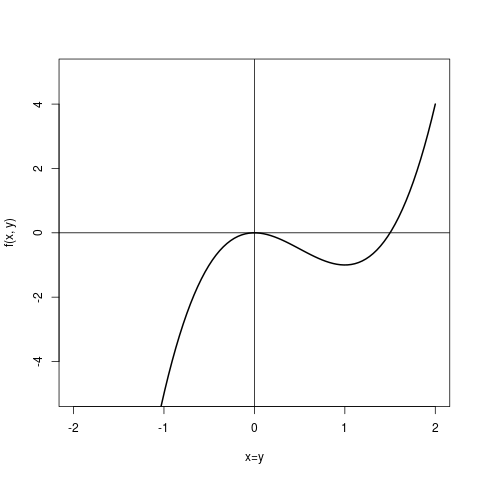
\includegraphics[width=.35\textwidth, trim=00 10 10 40, clip=]{ExempleOptimum-1ereBissectrice} &
        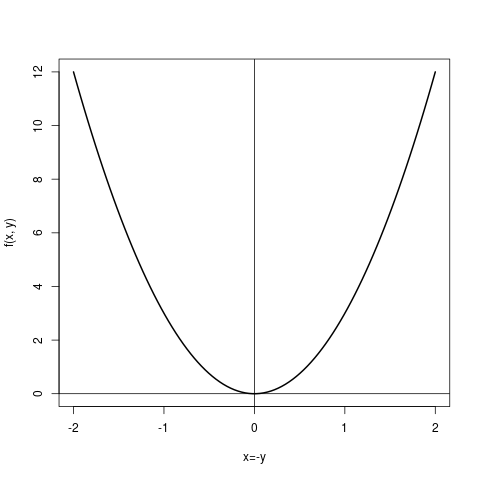
\includegraphics[width=.35\textwidth, trim=00 10 10 40, clip=]{ExempleOptimum-2emeBissectrice} \\
        $f(x, x) = 2x^3 - 3x^2$ & $f(x, -x) = 3x^2$
      \end{tabular}
      $$
      \item[\'Etude du point $b$ :] on a
      $$
      \nabla_b^2 f = \left[\begin{array}{rrr} 6 & & -3 \\ -3 & & 6 \end{array}\right]
      \qquad \Rightarrow \qquad 
      | \nabla_b^2 f | = 27 > 0, \qquad \tr(\nabla_b^2 f) = 12 > 0
      $$
      donc les deux valeurs propres de $\nabla_b^2 f$ sont positives : $b$ est donc un minimum.
    \end{description}
    Au total la surface d'équation $\{z = f(x, y)\}$ a l'aspect suivant
    $$
    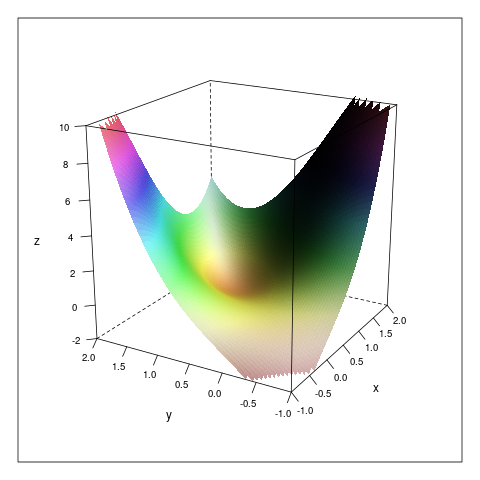
\includegraphics[width=.6\textwidth]{ExempleOptimum-surface}
    $$
  }
\end{enumerate}


%-------------------------------------------------------------------------------
% \section{Systèmes dynamiques}
%-------------------------------------------------------------------------------
\subsubsection{Système dynamique en $y^5$ \todo{}}
%-------------------------------------------------------------------------------

On souhaite déterminer les points d'équilibre (et leur nature) du système
$$
\dot y = F(y) = \mu y + 2 y^3 - y^5.
$$
On a 
$$
F(y) = y(\mu + y^2 - y^4)
$$
qui s'annule pour $y = 0$ et pour les solutions de $(\mu + 2 y^2 - y^4)$. En posant, $z = y^2$, $\mu + 2 z - z^2 = 0$ admet des solutions si $\Delta =  4(1 + \mu) \geq 0$, soit $\mu \geq -1$. Ces solutions sont alors $z^* = -1 \pm \sqrt{1+\mu}$. La seule solution possiblement positive est $z^* = -1 + \sqrt{1+\mu}$ et elle l'est ssi $\mu > 1$. \\
Le système admet donc un unique point fixe $x^*=0$ si $\mu < 1$ et un second point fixe $x^* = -1+\sqrt{1+\mu}$ si $\mu > 1$. \\
On a de plus
$$
F'(x) = \mu + 3 y^2 - 5y^4
$$
dont le signe est celui de $\mu$ pour $x=0$ et \todo{nature de $x^* = -1+\sqrt{1+\mu}$ si $\mu > 1$.}


%-------------------------------------------------------------------------------
\subsubsection{Modèle de Lotka-Volterra avec densité dépendance} 
%-------------------------------------------------------------------------------

\paragraph{Rappel.}
En notant 
\begin{itemize}
  \item $x(t)$ une variable proportionnelle au nombre de proies et
  \item $y(t)$ une variable proportionnelle au nombre de prédateurs,
\end{itemize}
le modèle Lotka-Volterra classique s'écrit, 
\begin{equation} \label{eq:LV}
\left\{\begin{array}{rcr}
        \dot x & = & r x (1 - y), \\ 
        \dot y & = & - m y (1 - x).
        \end{array}\right.
\end{equation}
Notamment, ce modèle admet deux points d'équilibre en $(x=0, y=0)$ et $(x=1, y=1)$.

\paragraph{Prise en compte d'une densité-dépendance.}
On considère ici un modèle de Lotka-Volterra avec densité dépendance. Plus précisément, en supposant le taux de croissance des proies égale à 1 ($r = 1$), on pose le modèle
\begin{equation} \label{eq:LVDD}
\left\{\begin{array}{rcr}
        \dot x & = & x (1 - y - ax), \\ 
        \dot y & = & - m y (1 - x), 
        \end{array}\right.
\end{equation}
où les paramètres $m$ et $a$ sont strictement positifs. 
% On remarque que le cas $a=0$ correspond au modèle de Lotka-Volterra classique (avec $r=1$).

\bigskip
\paragraph{Interprétation du modèle \eqref{eq:LVDD}.}
\begin{enumerate}
  \item Interpréter les paramètres $m$ et $a$ du modèle \eqref{eq:LVDD}.
  \solution{$m$ est le taux de mort des prédateurs en absence de proies (si $x(0)= 0$, $y(t) = y_0 e^{-mt}$). $a$ rend compte de la compétition entre les proies, c'est-à-dire de la limitation des ressources du milieu.}
  \item Déterminer les points d'équilibre du système \eqref{eq:LVDD}.
  \solution{
  L'isocline $\{\dot x = 0\}$ est $\Ical_x = \{x = 0\} \cup \{y = 1 - ax\}$ et l'isocline $\{\dot y = 0\}$ est $\Ical_y = \{y = 0\} \cup \{x = 1\}$. Les points d'équilibre sont donc $(0, 0)$, $(0, 1/a)$ et $(1, 1-a)$.}
  \item Expliquer la position du point d'équilibre $(x^*, y^*)$ non nul (c'est-à-dire pour lequel $x^*$ et $y^*$ sont non nuls) par rapport au point d'équilibre non nul du modèle de Lotka-Volterra classique \eqref{eq:LV}.
  \solution{L'équilibre non-trivial du modèle de Lotka-Volterra est le point $(1, 1)$. Le point d'équilibre des proies est conservé ($x^* = 1$), mais celui des prédateurs diminue $y^* = 1-a < 1$ : la contrainte imposée par le milieu au proies nuit, {\it in fine} à la population des prédateurs.}
\end{enumerate}

\bigskip
\paragraph{Questions intermédiaires (I).}
Soit la fonction $f: \Rbb^{*+} \mapsto \Rbb$, définie par $f(x) = \sqrt{x(x+1)} - x$.
\begin{enumerate}
  \setcounter{enumi}{3}
  \item Montrer que $f(x) > 0$. \label{q:LVDD-f1}
  \solution{On a $\sqrt{x(x+1)} > \sqrt{x^2} = x$, donc $f(x) > 0$.
  }
  \item Montrer que $f(x) < 1/2$. \label{q:LVDD-f2}
  \solution{On a
  $$
  f(x) < \frac12 
  \qquad \Leftrightarrow \qquad
  x(x+1) < \left(x + \frac12\right)^2
  \qquad \Leftrightarrow \qquad
  x^2 + x < x^2 + x + \frac14
  $$
  qui est toujours vrai.
  }
\end{enumerate}

\bigskip 
\paragraph{Questions intermédiaires (II).}
Soit la matrice $J^*$ définie par
\begin{equation} \label{eq:LVDD-Jstar}
  J^* = \left(\begin{array}{cc}
              -a & -1 \\ m(1-a) & 0
              \end{array}\right).
\end{equation}

\bigskip
\begin{enumerate}
  \setcounter{enumi}{5}
  \item Déterminer le polynôme caractéristique $P$ de $J^*$.
  \solution{$P(\lambda) = \lambda^2 + a \lambda + m(1-a)$.}
  %
  \item Montrer que les valeurs propres de $J^*$ sont réelles si et seulement si $a \geq a_1 = 2 f(m)$, où $f$ est la fonction définie en (I). 
  ({\sl On pourra étudier le discriminant $\Delta$ de $P$ comme une fonction de $a$.})
  \solution{La nature des valeurs propres de $J^*$ est donnée par le signe du discriminant de $P$ : $\Delta = \Delta(a) = a^2 + 4am - 4m$ qui est lui même un polynôme en $a$. \\
  Son discriminant est $\delta = 16m^2 + 16m = 16 m(m+1)$ est positif puisque $m$ est positif. 
  $\Delta(a)$ admet donc deux racines réelles:  $-2 (m + \sqrt{m(m+1)})$, qui est négative, et $a_1 = 2 (\sqrt{m(m+1)} - m) = 2f(m)$ qui est strictement positive d'après la question \ref{q:LVDD-f1}. 
  \\ $\Delta(a)$ est donc positif dès que $a \geq a_1 = 2 f(m)$ et $P$ admet alors deux racines réelles (égales si $a = a_1$). 
  }
  %
  \item Montrer que $a_1 < 1$ et que si $a > 1$, les valeurs propres de $J^*$ sont de signes différents. \label{q:racinePstar}
  \solution{
  La question \ref{q:LVDD-f2} nous assure que $a_1 = 2 f(m) < 1$, puisque $f(x) < 1/2$ pour tout $x \geq 0$. \\
  Si $a > a_1$, $P$ admet pour racines réelles $\lambda_1 = -(a +\sqrt{\Delta(a)})/2$, qui est toujours négative, et $\lambda_2 = (-a + \sqrt{\Delta(a)})/2$, qui est est positive dès que 
  $$
  \sqrt{\Delta(a)} \geq a
  \qquad \Leftrightarrow \qquad
  a^2 + 4am - 4m \geq a^2
  \qquad \Leftrightarrow \qquad
  a \geq 1.
  $$
  $J^*$ a donc des valeurs propres de racines distinctes dès que $a > 1 > a_1$. \\ 
  Alternativement, par les propriétés du polynôme caractéristique d'une matrice de $\Mcal_2$, $\lambda_1$ et $\lambda_2$ sont de même signe ssi $\lambda_1 \lambda_2 = |J^*| = m(1-a) > 0$, c'est-à-dire si $a <1$, puisque $m > 0$.
  }
\end{enumerate}
  

\bigskip
\paragraph{Stabilité du point d'équilibre non nul.}
On s'intéresse maintenant à la stabilité du point d'équilibre $(x^*, y^*)$ non nul. 
\begin{enumerate}
  \setcounter{enumi}{8}
  \item Déterminer la matrice jacobienne du système en un point $(x, y)$ quelconque.
  \solution{
  $$
  J = \left(\begin{array}{cc}
            -2ax + (1-y) & -x \\ my & m(x-1) 
            \end{array}\right).
  $$
  }
  \item En déduire que la matrice jacobienne en $(x^*, y^*)$ est égale à la matrice $J^*$ définie à l'équation \eqref{eq:LVDD-Jstar}.
  \solution{Direct.}
  \item \'Etudier la nature de l'équilibre $(x^*, y^*)$ en fonction de la position de $a$ par rapport aux deux valeurs seuils $a_1$ et $1$ : $a < a_1$, $a_1 < a < 1$ ou $a > 1$.
  ({\sl On ne s'attardera pas sur les cas limites $a = a_1$ et $a = 1$}.)
  \solution{
  \begin{description}
    \item[$a < a_1$ :] dans ce cas, $\Delta(a) < 0$ et les valeurs propres de $J*$ sont $\lambda_1$ et $\lambda_2$ calculées à la question \ref{q:racinePstar}, qui sont complexes mais dont les parties réelles sont négatives puisque $a > 0$. L'équilibre $(x^*, y^*)$ est donc un équilibre stable.
    \item[$a_1 < a < 1$ :] dans ce cas, $\Delta(a) > 0$ et les valeurs propres $\lambda_1$ et $\lambda_2$ sont toutes les deux réelles et négatives : l'équilibre $(x^*, y^*)$ est donc toujours stable.
    \item[$a > 1$ :] $\lambda_1$ est toujours négative mais $\lambda_2$ devient positive et $(x^*, y^*)$ devient alors instable.
  \end{description}
  Les figures suivantes donnent respectivement les parties réelles $Re(\lambda)$ et imaginaires $Im(\lambda)$  des valeurs propres $\lambda_1$ et $\lambda_2$ en fonction de $a$ pour $m=1/2$. 
  $$
  \begin{array}{c}
    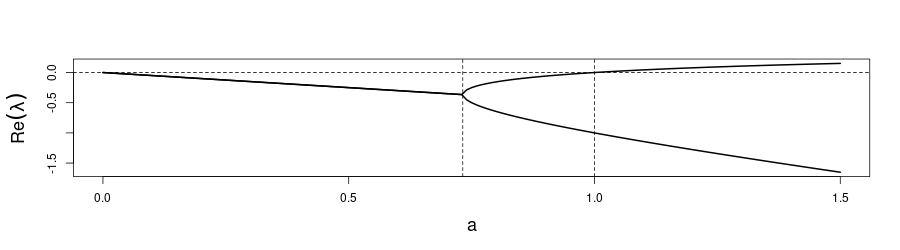
\includegraphics[width=.8\textwidth, trim=0 0 0 50, clip=]{LotkaVolterraDD-m0.5-eigenValueReal.png} \\
    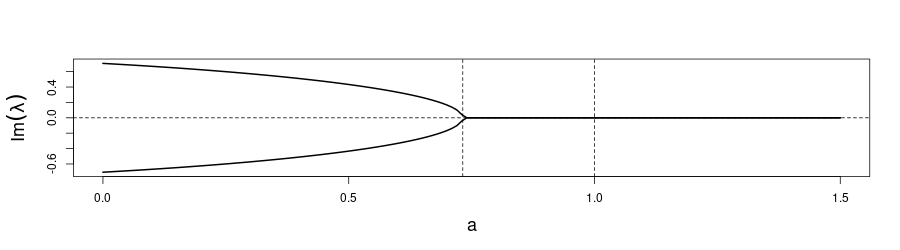
\includegraphics[width=.8\textwidth, trim=0 0 0 50, clip=]{LotkaVolterraDD-m0.5-eigenValueImaginary.png} 
  \end{array}
  $$
  La bifurcation se produit en $a = a_1$ et l'une des valeurs propres devient positive pour $a = 1$.
  }
\end{enumerate}

\bigskip
\paragraph{Trajectoires.}
Les trajectoires ($i$), ($ii$) et ($iii$) suivantes ont été obtenues par intégration numérique avec $m = 1/2$ et partant de l'état initial $(x_0 = 2,\;  y_0 = 3/2)$ pour trois valeurs de $a$ différentes :
$$
\begin{array}{ccc}
  (i) & (ii) & (iii) \\
  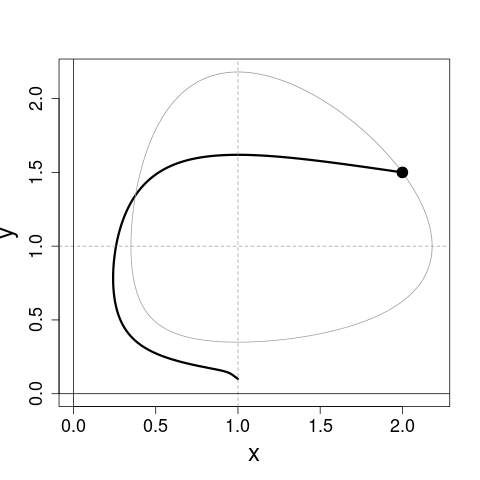
\includegraphics[width=.32\textwidth, trim=0 0 0 50, clip=]{LotkaVolterraDD-m0.5-a0.9.png} &
  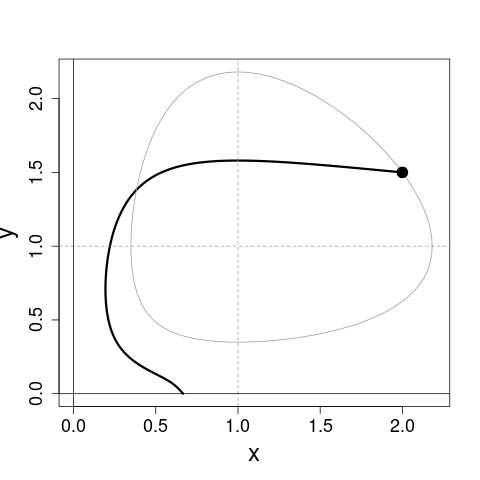
\includegraphics[width=.32\textwidth, trim=0 0 0 50, clip=]{LotkaVolterraDD-m0.5-a1.5.png} &
  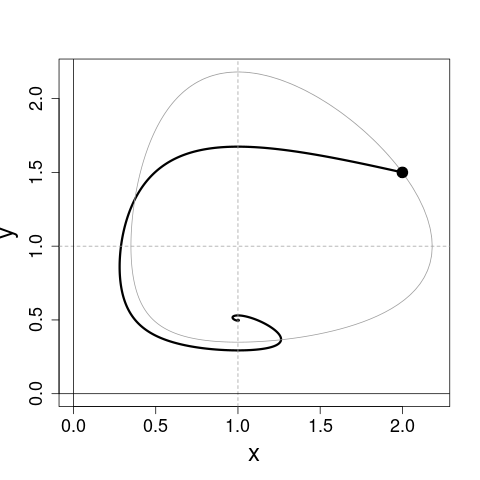
\includegraphics[width=.32\textwidth, trim=0 0 0 50, clip=]{LotkaVolterraDD-m0.5-a0.5.png}
\end{array}
$$
La courbe grise indique la trajectoire du modèle de Lotka-Volterra \eqref{eq:LV} sans densité-dépendance ($m = 1/2$, $a = 0$), partant du même point initial. Les repères grisés indiquent le point d'équilibre de ce même modèle \eqref{eq:LV}.

\begin{enumerate}
  \setcounter{enumi}{11}
  \item Associer chacune des trajectoires ($i$), ($ii$) et ($iii$) à l'une des trois valeurs de $a$ : $a = 1/2$, $a = 9/10$ et $a = 3/2$.
  \solution{On a dans ce cas $a_1 = 2 f(1/2) = \sqrt{3} - 1 \simeq 0.73$.
  \begin{description}
    \item[$a = 1/2 < a_1$ :] le système possède un équilibre stable en ($x^* = 1, y^* = 1/2$) et les valeurs propres de $J^*$ possèdent une partie imaginaire non nulle qui induit un enroulement autour de l'équilibre : on reconnaît la trajectoire ($iii$).
    \item[$a_1 < a = 9/10 < 1$ :] le système possède un équilibre stable en ($x^* = 1, y^* = 1/10$) mais les valeurs propres de $J^*$ sont réelles et négatives : le système tend vers l'équilibre sans enroulement : on reconnaît la trajectoire ($i$).
    \item[$a = 3/2 > a_1$ :] le système possède un équilibre instable en ($x^* = 1, y^* = -1/2$) que le système n'atteint jamais, du fait de l'extinction des prédateurs ($y(t) \to 0$) : on reconnaît la trajectoire ($ii$).
  \end{description}
  }
  \item Donner la limite de $x(t)$ quand $t$ tend vers l'infini dans le cas ($ii$).
  \solution{
  Dans ce cas, $y(t)$ tend vers 0 quand $t \to\infty$, le système \eqref{eq:LVDD-Jstar} devient donc simplement $\dot x = F(x)$ avec $F(x) = x (1 - ax)$. Ce système admet deux points d'équilibre en $x_1 = 0$ et $x_2 = 1/a$ et seul le second est stable (car $F'(x_1) > 0$ et $F'(x_2) < 0$). \\
  Après extinction des prédateurs, la population des proies tend donc vers un des équilibres 'nuls' : $(x_2 = 1/a = 2/3, y=0)$. Du fait de la densité-dépendance, la population des proies n'explose donc pas, contrairement au modèle de Lotka-Volterra classique.
  }
\end{enumerate}


%-------------------------------------------------------------------------------
% \section{Probabilités}
%-------------------------------------------------------------------------------
\subsubsection{Processus de Galton–Watson poissonnien} %-------------------------------------------------------------------------------
  On considère un processus de Bienaymé-Galton-Watson partant d'une population de taille 1 et dans laquelle le nombre de descendants par individu suit une loi géométrique $\Pcal(\lambda)$ :
  $$
  \Pr\{X = k\} = e^{-\lambda} \frac{\lambda^k}{k!}.
  $$
  \begin{enumerate}
    \item Rappeler le nombre moyen $m$ de descendants par individu.
    \solution{$m = \lambda$.}
    \item Déterminer la fonction génératrice $\phi$ du nombre de descendants par individu.
    \solution{Si $X \sim \Pcal(\lambda)$, 
    $$
    \phi(s) 
    = \Esp(s^X) 
    = e^{-\lambda} \sum_{k \geq 0} \frac{(\lambda s)^k}{k!} 
    = e^{\lambda(s-1)}.
    $$}
    \item A quelle condition sur $\lambda$ la probabilité d'extinction est-elle strictement inférieure à 1 ?
    \solution{Si $m = \lambda > 1$.}
    \item Pour quelle valeur de $\lambda$ as-t-on $q = 1/2$ ?
    \solution{On sait que $q$ vérifie $q = \phi(q)$, soit, 
    $$
    \lambda = \frac{\log q}{q - 1},
    $$
    soit, pour $q = 1/2$, $\lambda = 2 \log 2 \simeq 1.386$.}
  \end{enumerate}



%-------------------------------------------------------------------------------
%-------------------------------------------------------------------------------
\end{document}
%-------------------------------------------------------------------------------
%-------------------------------------------------------------------------------


